\Mysection{Motivation and Problem}
\begin{frame}{Motivation}
	\begin{itemize}
		\item International students must quickly understand many university systems and procedures.
		\item Relevant information is distributed across multiple channels:
		\begin{itemize}
			\item Moodle
			\item Mathplan timetable system
			\item university email activation
			\item orientation week procedures
			\item semester ticket
			\item examination systems
			\item administrative tasks in Germany
		\end{itemize}
		\item New students often do not know which source is authoritative for a specific question.
		\item As a result, onboarding becomes slower and more confusing than necessary.
	\end{itemize}
\end{frame}

\begin{frame}{Motivation: Information Fragmentation}
	\begin{center}
		\begin{tikzpicture}[
			node distance=1.5cm and 1.7cm,
			>=latex,
			every node/.style={font=\footnotesize, align=center},
			source/.style={rectangle, rounded corners, draw=blue!60!black, fill=blue!5, minimum width=2.6cm, minimum height=0.9cm},
			center/.style={circle, draw=HSELblau, fill=HSELhellblau!35, minimum size=2.0cm}
		]
			\node[center] (student) {Student};
			\node[source, above left=of student] (moodle) {Moodle};
			\node[source, above right=of student] (emails) {Emails};
			\node[source, left=of student] (pdfs) {PDF Guides};
			\node[source, right=of student] (web) {University\\Website};
			\node[source, below=of student] (office) {Coordination\\Office};

			\draw[->, thick] (moodle) -- (student);
			\draw[->, thick] (emails) -- (student);
			\draw[->, thick] (pdfs) -- (student);
			\draw[->, thick] (web) -- (student);
			\draw[->, thick] (office) -- (student);
		\end{tikzpicture}
	\end{center}

	\vspace{0.5em}
	\centering
	\footnotesize Information fragmentation during onboarding
\end{frame}

\begin{frame}{Current Problem}
	\begin{itemize}
		\item Students repeatedly ask operational questions during the first weeks of the semester.
		\item Answers already exist, but they are spread across different documents, portals, and contact points.
		\item This causes repeated explanations and slows down onboarding for both students and staff.
	\end{itemize}
\end{frame}

\begin{frame}{Current Problem: Typical Questions and Sources}
	\scriptsize
	\begin{tabular}{p{2.4cm} p{4.8cm} p{3.0cm}}
		\textbf{Category} & \textbf{Example Question} & \textbf{Current Source} \\
		\hline
		University Account & How do I activate email? & Orientation email \\
		Course Systems & How do I access Moodle? & IT documentation \\
		Timetable & How do I use Mathplan? & Moodle guide \\
		Administration & How do I get semester ticket? & University portal \\
		Exams & Where can I find transcript? & Examination office \\
	\end{tabular}
\end{frame}

\Mysection{Concept Proposal}

\begin{frame}{Proposed Solution}
	\begin{itemize}
		\item Concept: a \textbf{Local LLM-based Student Support Assistant}.
		\item The assistant should:
		\begin{itemize}
			\item answer student questions
			\item retrieve information from official documents
			\item guide users through university processes
			\item provide relevant links to resources
			\item cite the underlying source documents
		\end{itemize}
		\item The objective is not to replace staff, but to provide a first, structured support layer.
	\end{itemize}
\end{frame}

\begin{frame}{Proposed Solution: Knowledge Hub}
	\begin{center}
		\begin{tikzpicture}[
			node distance=1.1cm and 1.1cm,
			>=latex,
			every node/.style={font=\footnotesize, align=center},
			box/.style={rectangle, rounded corners, draw=blue!60!black, fill=blue!5, minimum width=2.8cm, minimum height=0.9cm},
			core/.style={rectangle, rounded corners, draw=HSELblau, fill=HSELhellblau!30, minimum width=3.1cm, minimum height=1.0cm}
		]
			\node[box] (student) at (0,0) {Student};
			\node[core] (assistant) at (4.0,0) {AI Assistant};
			\node[box] (emails) at (8.2,1.8) {Orientation\\Emails};
			\node[box] (moodle) at (8.2,0.6) {Moodle\\Documentation};
			\node[box] (guides) at (8.2,-0.6) {Administrative\\Guides};
			\node[box] (pages) at (8.2,-1.8) {University\\Resource Pages};

			\draw[->, thick] (student) -- (assistant);
			\draw[->, thick] (assistant) -- (emails);
			\draw[->, thick] (assistant) -- (moodle);
			\draw[->, thick] (assistant) -- (guides);
			\draw[->, thick] (assistant) -- (pages);
		\end{tikzpicture}
	\end{center}

	\vspace{0.5em}
	\centering
	\footnotesize Knowledge hub concept
\end{frame}

\begin{frame}{Example Interaction}
	\begin{columns}[T]
		\begin{column}{0.42\textwidth}
			\textbf{Example question}
			\begin{block}{Student Input}
				How do I activate my university email?
			\end{block}

			\vspace{0.4em}
			\textbf{Expected response structure}
			\begin{itemize}
				\item step-by-step instructions
				\item link to the activation portal
				\item explanation of required information
				\item citation of the source document
			\end{itemize}
		\end{column}
		\begin{column}{0.54\textwidth}
			\begin{center}
				\begin{tikzpicture}[
					>=latex,
					every node/.style={font=\scriptsize, align=left},
					bubbleq/.style={rectangle, rounded corners, draw=HSELblau, fill=HSELhellblau!25, text width=4.5cm, inner sep=6pt},
					bubblera/.style={rectangle, rounded corners, draw=blue!60!black, fill=blue!5, text width=4.8cm, inner sep=6pt}
				]
					\node[bubbleq] (q) at (0,0) {User question:\\How do I activate my university email?};
					\node[bubblera] (a) at (0,-2.2) {Assistant response:\\1. Open activation portal\\2. Enter student credentials\\3. Set password\\4. Confirm mailbox access};
					\node[bubblera] (s) at (0,-4.3) {Source reference:\\Orientation email + IT activation guide};
				\end{tikzpicture}
			\end{center}
		\end{column}
	\end{columns}
\end{frame}

\begin{frame}{System Concept}
	\begin{itemize}
		\item The system follows a retrieval-based architecture instead of relying only on model memory.
		\item The assistant first searches relevant university material, then generates an answer grounded in those sources.
		\item This improves traceability and supports source citation in responses.
	\end{itemize}

	\vspace{0.8em}
	\begin{center}
		\resizebox{0.96\textwidth}{!}{
			\begin{tikzpicture}[
				node distance=1.3cm and 0.8cm,
				>=latex, thick,
				every node/.style={font=\footnotesize, align=center},
				box/.style={rectangle, rounded corners, draw=blue!60!black, fill=blue!5, minimum width=2.1cm, minimum height=0.9cm}
			]
				\node[box] (q) {Student\\Question};
				\node[box, right=of q] (qp) {Query\\Processing};
				\node[box, right=of qp] (dr) {Document\\Retrieval};
				\node[box, right=of dr] (db) {Vector\\Database};
				\node[box, right=of db] (llm) {Local\\LLM};
				\node[box, right=of llm] (ans) {Answer with\\Source Citation};

				\draw[->] (q) -- (qp);
				\draw[->] (qp) -- (dr);
				\draw[->] (dr) -- (db);
				\draw[->] (db) -- (llm);
				\draw[->] (llm) -- (ans);
			\end{tikzpicture}
		}
	\end{center}
\end{frame}

\Mysection{Prototype and Deployment}

\begin{frame}{Prototype Implementation}
	\begin{itemize}
		\item The prototype is planned as a \textbf{local system} running on the \textbf{RTX 5090 GPU available in the lab}.
		\item This setup is suitable to demonstrate:
		\begin{itemize}
			\item local inference
			\item privacy-preserving architecture
			\item effective use of available GPU resources
		\end{itemize}
		\item The goal is a proof of concept for student support, not a production deployment.
	\end{itemize}
\end{frame}

\begin{frame}{Prototype Implementation: Local Architecture}
	\begin{center}
		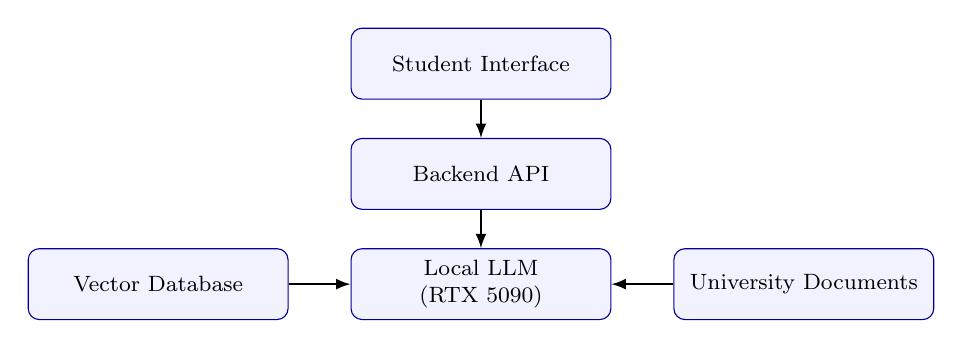
\begin{tikzpicture}[
			node distance=1.0cm,
			>=latex,
			every node/.style={font=\footnotesize, align=center},
			box/.style={rectangle, rounded corners, draw=blue!60!black, fill=blue!5, minimum width=3.3cm, minimum height=0.9cm}
		]
			\node[box] (ui) at (0,2.4) {Student Interface};
			\node[box] (api) at (0,1.0) {Backend API};
			\node[box] (llm) at (0,-0.4) {Local LLM\\(RTX 5090)};
			\node[box] (db) at (-4.1,-0.4) {Vector Database};
			\node[box] (docs) at (4.1,-0.4) {University Documents};

			\draw[->, thick] (ui) -- (api);
			\draw[->, thick] (api) -- (llm);
			\draw[->, thick] (db) -- (llm);
			\draw[->, thick] (docs) -- (llm);
		\end{tikzpicture}
	\end{center}
\end{frame}

\begin{frame}{Possible Deployment (Future Concept)}
\scriptsize
\begin{tabular}{p{2.7cm} p{3.9cm} p{3.2cm}}
\textbf{Access Method} & \textbf{Description} & \textbf{Comments} \\
\hline

Web Application & Browser-based chat interface accessible from any device & Can be linked from Moodle or shared via QR code \\

Messaging Bot & Chat interface via Telegram or WhatsApp & Familiar interface; mobile-friendly access \\

Internal Web App (Campus Network) & Web interface accessible only within university network & Can integrate with Moodle or internal systems \\

\end{tabular}
\end{frame}

\Mysection{Expected Value and Feedback}

\begin{frame}{Potential Benefits}
	\textbf{For Students}
	\begin{itemize}
		\item Faster answers to common questions (timetable, Moodle, email activation, semester ticket)
		\item Centralized access to important study information
		\item 24/7 access to guidance for administrative processes (potential feature)
	\end{itemize}

	\textbf{For Coordination Office}
	\begin{itemize}
		\item Reduced workload from repetitive onboarding queries
		\item Support available even when staff are not immediately reachable
		\item Better focus on complex student issues rather than routine guidance
	\end{itemize}

	\textbf{For University}
	\begin{itemize}
		\item Potential foundation for a university-wide digital student assistant
		\item Scalable architecture that could support other programs and departments
	\end{itemize}
\end{frame}


\begin{frame}{Questions and Feedback}
\begin{enumerate}
    \item \textbf{General feedback on the idea} \\
    Could this concept work as a project for \textbf{Project B under the “Local LLM Agent” topic}? 
    We would appreciate any feedback on whether this idea is appropriate for the course.

    \item \textbf{Scope of the Local LLM Agent} \\
    How broad should the scope of the assistant be? Should we focus specifically on the 
    \textbf{MBIDA + TM programs}, or consider a more general assistant for 
    \textbf{international students at the university}?
\end{enumerate}
\end{frame}

\begin{frame}{Questions and Feedback (cont.)}
\begin{enumerate}
    \setcounter{enumi}{2}

    \item \textbf{Type of prototype} \\
    What type of prototype would you prefer to see for this project?
    \begin{itemize}
        \item A \textbf{local prototype running on the RTX 5090 or a laptop}, mainly demonstrating the AI architecture and retrieval system
        \item Or a \textbf{simple web application} that students could potentially start using next semester
    \end{itemize}

    \item \textbf{Research directions and resources} \\
    Are there any \textbf{technical directions, research aspects, or resources} you would recommend exploring for this project?
\end{enumerate}
\end{frame}